\section{工具使用}

\subsection{杂项}
\par json格式的array中的element是保持顺序的(顺序敏感的),而其它类型不是顺序敏感的。
\par Eclipse中删除无用的import:《Ctrl+ Shift + O》 do it manually or Window -> Preferences -> Java -> Editor -> Save Actions -> Organize Imports to have it organized automatically whenever save a class。或者在Package Explorer窗口中,使用《Ctrl+ Shift + O》快捷键。
\par 安装Mate桌面环境后,会碰到没有声音的情况,此时可以删除pulseaudio,执行命令后重启机器。
\subsection{Linux Shell}
\par 使用nutch时,如果目录中文件太多,且包含了很多不需要的类型(如音频,视频),可使用rsync命令,保持源文件夹目录结构,同时只提取指定类型。
\begin{verbatim}
rsync -av --exclude='path1/exclude' --exclude='path2/exclude' [source] [dest]
rsync -av --include='*.shtml' --include='*.doc' --include='*.pdf' --include='*/' --exclude='*' /mnt/d data/
\end{verbatim}
\par 注意[source]与[source/]不同,前者表示拷贝source目录,后者表示拷贝目录下的内容。如果需要过滤的文件太多,可使用[--exclude-from=FILE]参数,其中FILE存储需过滤的文件或目录。也可过滤类型,如[--exclude=*/.svn*]。
\begin{verbatim}
sudo apt-get autoremove pulseaudio
\end{verbatim}
\par 标准输入stdin,标准输出stdout,标准错误stderr,其文件描述符分别为0,1,2。>默认为将标准输出(stdout)重定向到其它地方,2>\&1表示将标准错误输出(stderr)重定向到标准输出(stdout)。\&>file表示把标准输出(stdout)和标准错误(stderr)都输出到文件file中。特别注意,2>1表示将stderr重定向到文件1中,而非stdout。
\par let命令的替代表示形式是:((算术表达式))。例如,let 'j=i*6+2'等价于((j=i*6+2))。当表达式中有Shell的特殊字符时,必须用双引号或单引号将其括起来。例如,let ``val=a\textbar b''。如果不括起来,Shell会把命令行let val=a\textbar b中的''\textbar''看作管道符号,将其左右两边看成不同的命令,因此,将无法正确执行。 
\par linux中除了常见的读(r)、写(w)、执行(x)权限以外,还有3个特殊的权限,分别是setuid、setgid和stick bit。
\begin{verbatim}
[root@MyLinux ~]# ls -l /usr/bin/passwd /etc/passwd
-rw-r--r-- 1 root root  1549 08-19 13:54 /etc/passwd
-rwsr-xr-x 1 root root 22984 2007-01-07 /usr/bin/passwd
\end{verbatim}
\par /etc/passwd文件存放的各个用户的账号与密码信息,/usr/bin/passwd是执行修改和查看此文件的程序,但从权限上看,/etc/passwd仅有root权限的写(w)权,可实际上每个用户都可以通过/usr/bin/passwd命令去修改这个文件,于是这里就涉及了linux里的特殊权限setuid,正如-rwsr-xr-x中的s,setuid就是:让普通用户拥有可以执行“只有root权限才能执行”的特殊权限,setgid同理是让普通用户拥有“组用户”才能执行的特殊权限”。
\par /tmp目录是所有用户共有的临时文件夹,所有用户都拥有读写权限,这就必然出现一个问题,A用户在/tmp里创建了文件a,此时B用户看了不爽,在/tmp里把它给删了(因为拥有读写权限),那肯定是不行的。实际上不会发生这种情况,因为有特殊权限stick bit(粘贴位)权限,drwxrwxrwt中的最后一个t的意思是:除非目录的owner和root用户才有权限删除它,除此之外其它用户不能删除和修改这个目录。也就是说,/tmp目录中,只有文件的拥有者和root才能对其修改和删除,其他用户则不行,避免了上面所说的问题。
\par 如何设置以上特殊权限,如下所示,suid的二进制串为100,换算十进制为4,guid的二进制串为010,stick bit二进制串为001,换算成1。在一些文件设置了特殊权限后,字母不是小写的s或者t,而是大写的S和T,那代表此文件的特殊权限没有生效,是因为尚未赋予它对应用户的x权限。\\
\begin{minipage}{.5\linewidth}
\begin{verbatim}
setuid:chmod u+s xxx
setgid: chmod g+s xxx
stick bit : chmod o+t xxx
\end{verbatim}  
\end{minipage}
\begin{minipage}{.5\linewidth}
\begin{verbatim}
setuid:chmod 4755 xxx
setgid:chmod 2755 xxx
stick bit:chmod 1755 xxx
\end{verbatim}  
\end{minipage}
\subsection{git基本命令}
\par git add命令主要用于把要提交的文件的信息添加到索引库中,当使用\textbf{git commit}时,git将依据索引库中的内容来进行文件的提交。\textbf{git add <path>}表示add to index only files created or modified and not those deleted,因此\textbf{git add <path>}添加的文件不包括已经删除了的文件,<path>可以是文件也可以是目录。git不仅能判断出<path>中,修改(不包括已删除)了的文件,还能判断出新建的文件,并把它们的信息添加到索引库中。
\par \textsl{git add -u <path>}表示add to index only files modified or deleted and not those created,即把<path>中所有的tracked文件添加到索引库,它不会处理untracked的文件。\textsl{git add -A <path>}表示把<path>中所有的tracked文件和所有的untracked的文件信息添加到索引库。当省略<path>时,<path>等价于'./'(当前目录)。
\par 使用\textsl{git add ./}后,如果打算撤销这次添加,则使用命令:\textsl{git rm -r --cached ./}。如果忽略某些类型或某些目录时,可在.gitignore文件中添加内容,最后一行忽略\textsl{mapreduce/ESMapReduce/lib/}目录下的所有内容。
\begin{verbatim}
*.class
*.jar
*.ear
mapreduce/ESMapReduce/lib/
\end{verbatim}
\par git提交环节存在三大部分:\textsl{working tree,index file,commit}。working tree是工作所在的目录,每当在代码中进行了修改,working tree的状态就改变了。index file是索引文件,它是连接working tree和commit的桥梁,每当使用git add命令后,index file的内容就改变了,此时index file和working tree完成了同步。commit是代码的一次提交,只有完成提交,代码才真正地进入git仓库,使用git commit就是将index file内容提交到commit中。因此,\textbf{git diff}是查看working tree与index file的差别的,\textbf{git diff --cached}是查看index file与commit的差别的,\textbf{git diff HEAD}是查看working tree和commit的差别的(HEAD代表最近一次commit)。
\par 发生错误时,如果想回到此前的一个版本,命令为\textbf{git reset --soft}。使用\textbf{git log}命令,查看日志中有哪些commit以及commit的ID,最后使用命令\textbf{git reset commitID}回退到该版本。
\begin{verbatim}
git branch 查看本地有哪些分支
git branch -r 查看远程仓库有哪些分支
下载远程仓库(origin/1.2)到本地,分枝名同样为1.2
git checkout -b 1.2 origin/1.2
git checkout master 切换到master分支
git checkout 1.2 切换到1.2分支
\end{verbatim}
\subsubsection{不同仓库的操作}
\begin{enumerate}[(1)]
\item git branch -r 查看远程仓库有哪些分支
\item git clone gitosis@192.168.2.4:xhw/soul-client
\item 执行<git init>,修改当前目录下的<.git/config>文件,将xhw改为liubo
\item 执行<git remote -v>查看有哪些远程仓库
\item git remote add smq gitosis@192.168.2.4:/smq/soul-client
\item git remote add chen gitosis@192.168.2.4:/chengjie/soul-client
\item 再次执行<git remote -v>查看远程仓库有何更新
\item 执行<git pull smq master>拉取更新
\end{enumerate}
\subsection{Maven入门}
\begin{enumerate}[(1)]
\item 配置maven环境,最主要的是设置环境变量:M2\_HOME,将其设置为maven安装目录,例子目录为:/usr/share/maven;
\item 修改仓库位置,仓库用于存放平时项目开发依赖的所有jar包。例子仓库路径:/opt/maven/repo,为设置仓库路径,必须修改\textbf{\${M2\_HOME}/conf}目录下的setting.xml文件。\\
<localRepository>/opt/maven/repo</localRepository> \\
在shell中输入并执行mvn help:system,如果没有错误,在仓库路径下应该多了些文件,这些文件是从maven的中央仓库下载到本地仓库的。
\item 创建maven项目,通过maven命令行方式创建一个项目,命令为:\textbf{mvn archetype:create -DgroupId=com.mvn.test -DartifactId=hello -DpackageName=com.mvn.test -Dversion=1.0}\\
由于第一次构建项目,所有依赖的jar包都要从maven的中央仓库下载,所以需要时间等待。做完这一步后,在工程根目录下应该有个pom.xml文件,其中groupId,artifactId和version比较常用。
\begin{itemize}
\item project:pom.xml文件的顶层元素;
\item modelVersion:指明POM使用的对象模型的版本,这个值很少改动。
\item groupId:指明创建项目的小组的唯一标识。GroupId是项目的关键标识,此标识以组织的完全限定名来定义。如org.apache.maven.plugins是所有Maven插件项目指定的groupId。
\item artifactId:指明此项目产生的主要产品的基本名称。项目的主要产品通常为一个jar包,源代码包通常使用artifactId作为最后名称的一部分。典型的产品名称使用这个格式:<artifactId>-<version>.<extension>(比如:myapp-1.0.jar)。
\item version:项目产品的版本号。Maven帮助你管理版本,可以经常看到SNAPSHOT这个版本,表明项目处于开发阶段。
\item name:项目的显示名称,通常用于maven产生的文档中。
\item url:指定项目站点,通常用于maven产生的文档中。
\item description:描述此项目,通常用于maven产生的文档中。
\end{itemize}
\item 项目hello已经创建完成,但它并不是eclipse所需要的项目目录格式,需要把它构建成eclipse可以导入的项目。进入到刚创建的项目目录(\textasciitilde/workspace/hello),执行:\textbf{mvn clean}(告诉maven清理输出目录target),然后执行\textbf{mvn compile}(告诉maven编译项目main部分的代码,或者两步合成一步\textbf{mvn clean compile}),此次仍会下载jar包到仓库中。编译后,项目的目录结构并不可以直接导入到Eclipse,需执行命令:\textbf{mvn eclipse:eclipse},命令执行完成后就能import到Eclipse。
\begin{figure}[htbp]
\centering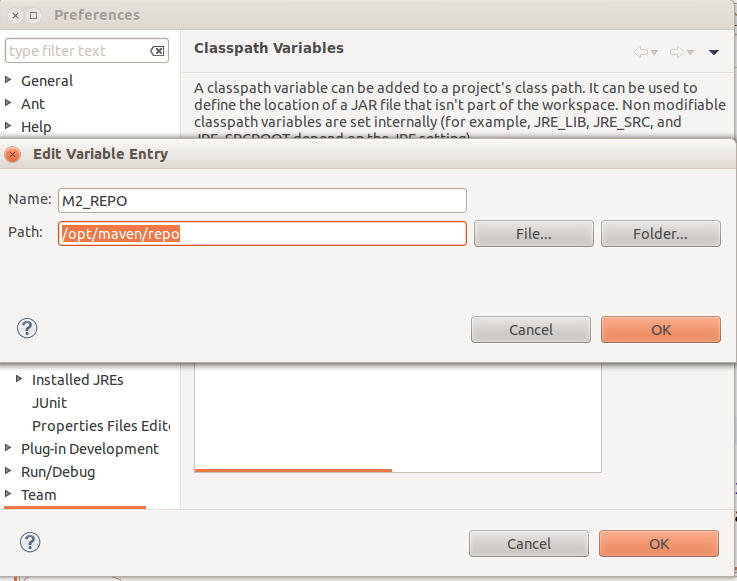
\includegraphics[width=0.7\linewidth]{figures/maven-1.png}
\caption{Eclipse配置Maven仓库路径}\label{fig-maven-1}
\end{figure} 
\item 打开eclipse,在其中配置maven仓库路径,配置路径为:Window-->Perferences-->java-->Build Path-->Classpath Variables,新建变量(M2\_REPO)的类路径,如图\ref{fig-maven-1}示。
\item 包的更新与下载,如果发现junit版本比较旧,想换成新版本,修改项目下的的pom.xml文件为
\begin{verbatim}
<dependencies>
  <dependency>
     <groupId>junit</groupId>
     <artifactId>junit</artifactId>
     <version>4.8.1</version>
     <scope>test</scope>
  </dependency>
</dependencies>
\end{verbatim}
就可改变junit的版本号,在以后的maven操作中,maven会自动下载依赖的jar包。Maven中央仓库地址为http://search.maven.org,假如想下载struts的jar包,可在url内搜索struts。
\item 某些jar包可能位于远程机器上,因此需要配置maven仓库,配置仓库代码如下,其中的id属性无特别含义,仅用于标识仓库。当下载完某个jar包后,其在本地仓库的相对路径形如<groupId>/<artifactId>/<version>/*.jar,例如:/opt/maven/repo/org/ansj/tree\_split/1.0.1/tree\_split-1.0.1.jar。
\begin{verbatim}
<repositories>
  <repository>
    <id>ansj-maven-repo</id>
    <url>https://raw.github.com/ansjsun/mvn-repo/gh-pages</url>
  </repository>
  <repository>
    <id>remote-maven-repo</id>
    <url>http://search.maven.org</url>
  </repository>
</repositories>
\end{verbatim}
\item 有时候Maven访问很慢,可在settings.xml里重新设置中央仓库的镜像,中央仓库的默认地址为:http://repo.maven.apache.org/maven2/
\begin{verbatim}
<mirrors>
 <mirror>
   <id>ibiblio</id>
   <mirrorOf>central</mirrorOf>
   <name>Human Readable Name for this Mirror.</name>
   <url>http://mirrors.ibiblio.org/maven2</url>
 </mirror>
</mirrors>
\end{verbatim}
\end{enumerate}
\par 打算执行maven工程下某个类时,例如test目录下的某个类,执行命令如下:\textbf{mvn exec:java -X -Dexec.mainClass="org.ansj.liubo.test.test"  -Dexec.classpathScope=test},其中的classpathScope=test告诉maven执行test类,而非main类。执行test部分的某些类之前,必须执行\textbf{mvn test-compile},以编译test部分的代码(test类中必须有main函数),如没有编译,则执行会报错。当准备向执行类添加参数时,使用如下命令。
\begin{verbatim}
mvn exec:java -Dexec.mainClass="org.elasticsearch.application.WebDemo"
  -Dexec.args="/mnt/f/tmp/content.txt /mnt/f/tmp/result3.txt"  
  -Dexec.classpathScope=test
## 如下命令执行TestNG框架中的test类(没有main函数)
mvn test -Dtest="com.soul.elasticsearch.test.OfficialDataTest"
\end{verbatim}
\subsection{Maven常用插件}
\par Maven本质上是一个插件框架,其核心并不执行任何具体的构建任务,所有这些任务都交给插件完成,例如编译源代码由maven-compiler-plugin完成。进一步说,每个任务对应一个插件,每个插件会有一个或者多个目标(goal),例如maven-compiler-plugin的compile目标用来编译src/main/java/目录的code,而testCompile目标则用来编译src/test/java/目录的code。
\par 用户可通过两种方式调用Maven插件目标。第一种方式是将插件目标与生命周期阶段(lifecycle phase)绑定,这样用户在命令行只输入了生命周期阶段,例如Maven默认将maven-compiler-plugin的compile目标与compile生命周期阶段绑定,因此命令\textbf{mvn compile}实际上先定位到compile这一生命周期阶段,然后再根据绑定关系调用maven-compiler-plugin的compile目标。第二种方式是直接在命令行指定要执行的插件目标,例如\textbf{mvn archetype:generate}就表示调用maven-archetype-plugin的generate目标,这种带冒号的调用方式与生命周期无关。
\par Maven有两个插件列表,第一个列表GroupId为org.apache.maven.plugins,这里的插件最为成熟,具体地址为:http://maven.apache.org/plugins/index.html。第二个列表的GroupId为org.codehaus.mojo,这里的插件没有那么成熟,但也十分有用,地址为:http://mojo.codehaus.org/plugins.html。
\par 为使项目结构更为清晰,Maven区别对待Java代码文件和资源文件,maven-compiler-plugin用来编译java代码,maven-resources-plugin则用来处理resource文件。默认的资源文件目录是src/main/resources。很多用户会添加额外的资源文件目录,这个时候就可以通过配置maven-resources-plugin来实现。此外,资源文件过滤也是Maven的一大特性,可以在资源文件中使用\textbf{\${propertyName}}形式的Maven属性,然后配置maven-resources-plugin以开启对资源文件的过滤,之后就可以通过命令行或者Profile,针对不同环境传入不同的属性值,以实现灵活构建。
\par 由于历史原因,Maven用于执行测试的插件不是maven-test-plugin,而是maven-surefire-plugin。其实大部分时间内,只要测试类遵循通用的命令约定(以Test结尾、以TestCase结尾、或者以Test开头),就几乎不用知晓该插件是否存在。想要跳过测试、排除某些测试类、或者使用一些Test特性时,了解maven-surefire-plugin的一些配置选项就很有用了。例如\textbf{mvn test -Dtest=FooTest}这样一条命令的效果是仅运行FooTest测试类,这是通过控制maven-surefire-plugin的test参数实现的。
\par Maven默认只允许指定一个主Java代码目录和一个测试Java代码目录,虽然这是一个应当尽量遵守的约定,但偶尔用户还是希望能够指定多个源码目录,build-helper-maven-plugin的add-source目标就服务于这个目的,通常它被绑定到默认生命周期的generate-sources阶段以添加额外的源码目录。这种做法是不推荐的,因为它破坏了Maven的约定,而且可能会遇到其他严格遵守约定的插件工具无法正确识别额外的source目录。build-helper-maven-plugin的另一个非常有用的目标是attach-artifact,使用该目标你可以以classifier的形式选取部分项目文件生成附属构件,并同时install到本地仓库,也可以deploy到远程仓库。
\par exec-maven-plugin很好理解,顾名思义,它能让你运行任何本地的系统程序,在某些特定情况下,运行一个Maven外部的程序可能就是最简单的问题解决方案,这就是exec:exec的用途,当然,该插件还允许你配置相关的程序运行参数。除了exec目标之外,exec-maven-plugin还提供了一个java目标,该目标要求你提供一个mainClass参数,然后它能够利用当前项目的依赖作为classpath,在同一个JVM中运行该mainClass。有时候,为了简单的演示一个命令行Java程序,可以在pom.xml中配置好exec-maven-plugin的相关运行参数,然后直接在命令运行\textbf{mvn exec:java}以查看运行效果。
\par 进行Web开发时,打开浏览器对应用进行手动的测试几乎是无法避免的,这种测试方法通常就是将项目打包成war文件,然后部署到Web容器中,再启动容器进行验证,这显然十分耗时。为了帮助开发者节省时间,jetty-maven-plugin应运而生,它完全兼容Maven项目的目录结构,能够周期性地检查源文件,一旦发现变更后自动更新到内置的Jetty Web容器中。做一些基本配置后(例如Web应用的contextPath和自动扫描变更的时间间隔),只要执行\textbf{mvn jetty:run},然后在IDE中修改代码,代码经IDE自动编译后产生变更,再由jetty-maven-plugin侦测到后将更新写入到Jetty容器,这时就可以直接测试Web页面。需要注意的是,jetty-maven-plugin并不是宿主于Apache或Codehaus的官方插件,因此使用的时候需要额外的配置settings.xml的pluginGroups元素,将org.mortbay.jetty这个pluginGroup加入。
\par 当项目包含大量模块的时候,集体更新版本就变成一件烦人的事情,versions-maven-plugin提供了很多目标帮助你管理Maven项目的各种版本信息。例如最常用的命令\textbf{mvn versions:set -DnewVersion=1.1-SNAPSHOT}就能帮助你把所有模块的版本更新到1.1-SNAPSHOT。该插件还提供了其他一些很有用的目标,display-dependency-updates能告诉你项目依赖有哪些可用的更新,类似的display-plugin-updates能告诉你可用的插件更新,use-latest-versions能自动帮你将所有依赖升级到最新版本。最后,如果对所做的更改满意,则可以使用\textbf{mvn versions:commit}提交,不满意的话也可以使用\textbf{mvn versions:revert}进行撤销操作。
\subsection{Building a Self-Contained Hadoop Job}
\par Non-trivial Hadoop jobs usually have dependencies that go beyond those provided by the Hadoop runtime environment. That means, if your job needs additional libraries you have to make sure they are on Hadoop’s classpath as soon as the job is executed. This article shows how you can build a self-contained job JAR that contains all your dependencies.
\par The Hadoop runtime environment expects additional dependencies inside a lib directory. That’s where we need Maven’s Assembly plugin: Using the plugin, we create a JAR that contains the project’s resources (usually just your job’s class files) and a lib directory with all dependencies that are not on Hadoop’s classpath already.
\par First of all, we create an assembly descriptor file (put it in {\color{red}src/main/assembly/hadoop-job.xml}). Note that we collect all dependencies on the runtime scope but exclude the project’s artifact. Instead, we add the artifact unpacked which is a little surprising. If we didn’t do that, Hadoop would look for our dependencies inside the project’s artifact JAR and not inside the surrounding assembly JAR's lib directory. For the whole mechanism to work, the class you set in your job driver via Job.setJarByClass() must be from your project, not from your dependencies.
\begin{verbatim}
<assembly>
  <id>job</id>
  <formats>
    <format>jar</format>
  </formats>
  <includeBaseDirectory>false</includeBaseDirectory>
  <dependencySets>
    <dependencySet>
      <unpack>false</unpack>
      <scope>runtime</scope>
      <outputDirectory>lib</outputDirectory>
      <excludes>
        <exclude>${groupId}:${artifactId}</exclude>
      </excludes>
    </dependencySet>

    <dependencySet>
      <unpack>true</unpack>
      <includes>
        <include>${groupId}:${artifactId}</include>
      </includes>
    </dependencySet>
  </dependencySets>
</assembly>
\end{verbatim}
\par Inside the POM's dependency section, we set Hadoop to the {\color{red}provided} scope,这样的话,Hadoop相关的jar包就不会被打包。
\begin{verbatim}
<dependencies>
  <dependency>
    <groupId>org.apache.hadoop</groupId>
    <artifactId>hadoop-core</artifactId>
    <version>2.0.5-alpha</version>
    <scope>provided</scope>
  </dependency>
</dependencies>
\end{verbatim}
\par Setting the assembly JAR's Main class is optional, but makes the job more user friendly because you don’t have to specify the class name explicitly for each run. You can now build your job JAR:
\begin{verbatim}
mvn clean package
\end{verbatim}
\par Your self-contained job JAR is the file in target ending with -job.jar. Run it using Hadoop’s jar sub-command: 
\begin{verbatim}
hadoop jar ./target/releases/soul_seg-0.3-job.jar /hdfs
\end{verbatim}
\par 使用上述命令打包时,将会运行test目录下的测试类,十分耗时。为此,使用如下命令跳过测试。
\begin{verbatim}
mvn clean package -Dmaven.test.skip=true
\end{verbatim}
\subsection{构造Java后台程序}
\par Lately I have been writing a Java program that needs to run in the background (like a daemon). These ideas probably only work in a Unix environment but they have been tested on Linux and Solaris. So you have your program and you want to start it such that it will not be killed when you log out of the shell in which you start it. You could use \textbf{nohup}, but \textbf{nohup} redirects the standard out and error to files, which is annoying because you are writing all output to a log file anyway. 
\begin{verbatim}
java -jar target/soul_seg-0.3.jar  <&- 1>/dev/null 2>&1 &
其中,<&-关闭标准输入,1>/dev/null 2>&1将标准输入重定向到/dev/null,最后一个&挂起该进程。
\end{verbatim}
\par 上面的命令runs the program in the background, closes standard in, and redirects standard out and error to the /dev/null. By closing standard in to the process the shell will not kill the program when it exits and it is running in the background so it will not interfere with other actions we might want to perform within this shell.
\par 但后台程序发生错误时,上述方法不会提示,如当监听端口被占用时,因此,重定向stdout和stderr不合适。The solution is to have the Java program detach from standard out and error once its startup is complete. So we will create a method called daemonize() that we will call just before entering the infinite loop that is the main program logic.
\begin{verbatim}
static public void daemonize() {
   System.out.close();//先关闭标准输出
   System.err.close();//先关闭标准错误输出
   final String pidFile = "/tmp/a/pidFile";
   File fPidFile = new File(pidFile);
   FileOutputStream oStream = new FileOutputStream(fPidFile);
   oStream.write(Long.toString(JvmInfo.jvmInfo().pid()).getBytes());
   oStream.close();
   fPidFile.deleteOnExit();
}
static public void main(String[] args) {
   try {
       // do sanity checks and startup actions
       daemonize();
   }
   catch (Throwable e)  {
       System.err.println("Startup failed.");
       e.printStackTrace();
   }
   // do infinite loop
}
\end{verbatim}
\par Now that the program is completely detached from the shell ,the only way to stop it is by killing the process. However, to do that you need to know the pid. 获取进程ID依赖于Java系统库,在daemonize()函数中,将进程ID保存在文件中(一般在/tmp目录下)。fPidFile.deleteOnExit()表示,当进程崩溃或关闭时,自动删除文件。
